% Created 2018-03-29 Thu 13:32
\documentclass[11pt]{article}
\usepackage[utf8]{inputenc}
\usepackage[T1]{fontenc}
\usepackage{fixltx2e}
\usepackage{graphicx}
\usepackage{longtable}
\usepackage{float}
\usepackage{wrapfig}
\usepackage{rotating}
\usepackage[normalem]{ulem}
\usepackage{amsmath}
\usepackage{textcomp}
\usepackage{marvosym}
\usepackage{wasysym}
\usepackage{amssymb}
\usepackage{hyperref}
\usepackage{minted}
\tolerance=1000
\author{Timothy Schwieg}
\date{\today}
\title{Econometrics Homework 6}

\begin{document}

\maketitle


\section{Question 1}
\label{sec-1}
$$f_Y(y|\theta) = \theta \exp( - \theta y ) \quad y > 0, \theta > 0$$
\subsection{a}
\label{sec-1-1}
Define:
$\hat{\theta} = g(M_1) = \frac{1}{M_1} = \frac{ N }{ \sum_{n=1}^N Y_n }$
Taking a second-order Taylor-Series expansion of $\hat{\theta}$ gives us:
$$g(M_1) = g( \mu_1(\theta^0) ) + g'(\mu_1(\theta^0))( M_1 - \mu_1(\theta^0) ) + \frac{1}{2}g''( \mu_1(\theta^0) )(M_1 - \mu_1(\theta^0) )^2 + R_3$$
Ignoring the remainder, and applying $g(M_1) = \frac{1}{M_1}$
$$\mathbb{E}[\hat{\theta}] = \theta^0 + \frac{2 \theta^0 V(Y)}{2N} = \frac{(N+1)\theta^0}{N}$$
The bias of $\hat{\theta}$ is given by:
$\mathbb{E}[\hat{\theta}] - \theta^0 = \frac{\theta^0}{N}$

A table representing the percentage of bias as a function of the
sample size N is given below. The first and third rows are the sample
size, and the second and fourth rows are the bias as a percentage.

\begin{center}
\begin{tabular}{|r|r|r|r|r|r|r|r|r|r|}\hline
5 & 10 & 15 & 20 & 25 & 30 & 35 & 40 & 45 & 50\\\hline
20 & 10 & 6.67 & 5 & 4 & 3.33 & 2.86 & 2.5 & 2.22 & 2\\\hline
55 & 60 & 65 & 70 & 75 & 80 & 85 & 90 & 95 & 100\\\hline
1.82 & 1.67 & 1.54 & 1.43 & 1.33 & 1.25 & 1.18 & 1.11 & 1.05 & 1\\\hline
\end{tabular}
\end{center}

\subsection{b}
\label{sec-1-2}

To establish the bias using the jackknife, first we define $\bar{
\hat{ \theta } } = \frac{1}{N} \sum_{n=1}^N \hat{ \theta}_{-n}$ Our estimate of the bias
is therefore: 

$$\widehat{ \text{Bias}( \hat{\theta} ) } = (N-1)[ \bar{ \hat{ \theta } } - \hat{ \theta } ]$$

\subsection{c}
\label{sec-1-3}

\begin{minted}[mathescape, fontsize=\small, xleftmargin=0.5em]{julia}
using Distributions
using Plots

J = 1000000

jackThetaBias = Vector{Float64}(J)
deltaThetaBias = Vector{Float64}(J)
trueBias = Vector{Float64}(J)


for j = 1:J

    N = 25

    sims = rand( Exponential(1), N )

    sumSims = sum( sims )
    jackThetaHat = Vector{Float64}(N)
    for i = 1:N
        jackThetaHat[i] = (N-1)/(sumSims - sims[i])
    end

    jackThetaBias[j] = (N-1)*( mean( jackThetaHat) - (1.0 /mean( sims)))

    #Delta method version
    deltaThetaBias[j] = 1.0/ sumSims

    trueBias[j] =  1.0 / mean( sims) - 1.0
end
pyplot()

jackKnifeDev = jackThetaBias .- trueBias
deltaDev = deltaThetaBias .- trueBias

#Average of jackKnifeDev:
println( mean( abs.(jackKnifeDev)) )
\end{minted}
\begin{minted}[fontsize=\small, xleftmargin=0.5em, mathescape, frame = leftline]{text}
0.16283567280038763
\end{minted}

\begin{minted}[mathescape, fontsize=\small, xleftmargin=0.5em]{julia}
#Average deviation of delta method from true bias
println( mean( abs.(deltaDev) ) )
\end{minted}
\begin{minted}[fontsize=\small, xleftmargin=0.5em, mathescape, frame = leftline]{text}
0.1622106416188522
\end{minted}

\begin{minted}[mathescape, fontsize=\small, xleftmargin=0.5em]{julia}
#Standard deviation of the deviations
println( std( jackKnifeDev))
\end{minted}
\begin{minted}[fontsize=\small, xleftmargin=0.5em, mathescape, frame = leftline]{text}
0.20893818911288065
\end{minted}

\begin{minted}[mathescape, fontsize=\small, xleftmargin=0.5em]{julia}
#Standard deviation of the deviations
println( std( deltaDev))
\end{minted}
\begin{minted}[fontsize=\small, xleftmargin=0.5em, mathescape, frame = leftline]{text}
0.20841208969566477
\end{minted}

\begin{minted}[mathescape, fontsize=\small, xleftmargin=0.5em]{julia}

#MSE of jackknife


#Plot them together
histogram( [jackKnifeDev, deltaDev],
line=(3,0,:green), fillcolor=[:red :black], fillalpha=0.5, show=true,
legend=:none)
\end{minted}
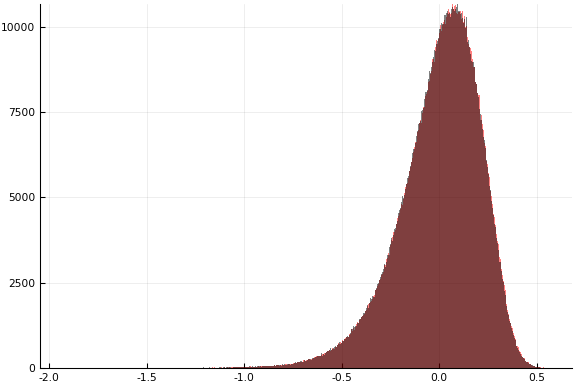
\includegraphics[width=\linewidth]{figures/Schwieg_HW6_1_1pdf}


It appears that the delta method is marginally better than the
jackknife at estimating the bias, at least for this function. From the
histogram it is hard to see any difference between them, with their
histograms pretty much occupying the same space.



\section{Question 2}
\label{sec-2}

\subsection{a}
\label{sec-2-1}
First we may note that $h(\beta)$ is continuous for all values of beta.

Since it is known that $\hat{\beta} \to \beta^0$, we can apply Slutsky's
theorem to $h( \hat{ \beta } )$ to see that plim $h( \hat{ \beta } ) =
plim \hat{\beta}_3 + plim \hat{\beta}_2  plim \hat{\beta}_4$ This is equal to
$\beta_{\text{3}} + \beta_{\text{2}} \beta_{\text{4}} = h( \beta^{\text{0}} )$ and we
can see that $h( \hat{ \beta } )$ is a consistent estimator of $h(
\beta^{0} )$.

Since it is known that $\hat{ \beta } \sim N( \beta^0, \mathbb{V}(\hat{\beta}) )$, we
may apply the multivariate delta method to get the asymptotic
distribution. Therefore $\sqrt{N} ( h( \hat{\beta} ) - h( \beta^0 ) ) \sim N( 0,
\nabla h( \hat{\beta} )^T \mathbb{V}( \hat{\beta} ) \nabla h( \hat{\beta} ) )$
asymptotically.



\subsection{b}
\label{sec-2-2}
Since h is not a linear function of $\beta$, we need a Wald statistic for
non-linear hypothesis, which will make use of the $\delta$ method.

We will use the non-linear Wald statistic. This takes the form of: 


$$ h(\hat{\theta}) [ h'( \hat{\theta} ) \mathbb{ V }( \hat{ \beta} ) h'( \hat{\theta} ) ]^{-1} h( \hat{\theta} ) \sim \chi^2 ( 1 )$$

\subsection{c}
\label{sec-2-3}
The advantage of using the Wald Statistic over the LR and LM tests is
that it does not require using constrained optimization. Both the LR
and the LM test would require that, which can be computationally
arduous. However, the statistic is limited because it handles
non-linearity by using the $\delta$ method, which is simply a first order
approximation of the result, and misses out on a lot of information
that can be conveyed by curvature and other higher order information.

The Wald test also has a slower rate of convergence than the likelihood
ratio test, since it converges at a rate of $O( \frac{ 1} {\sqrt{N} } )$

\end{document}